\section{Course Introduction}

\subsection{layers of abstraction}
\layersHighlighting{none}

\subsection{C}
\layersHighlighting{hll}

\usetikzlibrary{shapes.callouts}

\begin{frame}{why C?}
    \begin{itemize}
    \item \textit{almost} a subset of C++
        \begin{itemize}
        \item notably removes classes, new/delete, iostreams
        \item other changes, too, so C code often not valid C++ code
        \end{itemize}
    \item \myemph{direct\tikzmark{direct} correspondence} to assembly
    \end{itemize}
    \begin{tikzpicture}[overlay,remember picture]
        \onslide<2|handout:0>{
            \node[my callout=direct,align=left] {Should help you understand machine! \\
                                     Manual translation to assembly};
        }
        \onslide<3|handout:0>{
            \node[my callout=direct,align=left] {But ``clever'' (optimizing) compiler \\
                                     might be confusingly indirect instead};
        }
    \end{tikzpicture}
\end{frame}



\begin{frame}{homework: C environment}
    \begin{itemize}
    \item get Unix-like environment with a C compiler
    \item will have department accounts, hopefully by end of week
        \begin{itemize}
        \item portal.cs.virginia.edu or NX
        \item instructions off course website (Collab)
        \end{itemize}
    \item some other options:
        \begin{itemize}
        \item Linux (native or VM)
            \begin{itemize}
            \item 2150 VM image should work
            \end{itemize}
        \item most assignments can Windows Subsystem for Linux natively
        \item most assignments can use OS X natively
            \begin{itemize}
            \item notable exception: next week's lab+homework
            \end{itemize}
        \end{itemize}
    \end{itemize}
\end{frame}

\begin{frame}{assignment compatibility}
    \begin{itemize}
    \item supported platform: department machines
    \item many use laptops 
    \item trouble? we'll say to use department machines
    \vspace{.5cm}
    \item most assignments: C and Unix-like environment
    \item also: tool written in Rust --- but we'll provide binaries
        \begin{itemize}
        \item previously written in D + needed D compiler
        \end{itemize}
    \end{itemize}
\end{frame}


\subsection{assembly}

\layersHighlighting{asm}

\begin{frame}{X86-64 assembly}
    \begin{itemize}
    \item in theory, you know this (CS 2150)
    \item in reality, \ldots{}
    \end{itemize}
\end{frame}


\subsection{machine code}
\layersHighlighting{machineCode}

\begin{frame}{Y86-64??}
    \begin{itemize}
    \item Y86: our textbook's X86-64 subset
        \begin{itemize}
        \item hope: leverage 2150 assembly knowledge
        \end{itemize}
    \item much simpler than real X86-64 encoding
        \begin{itemize}
        \item (which we will not cover)
        \end{itemize}
    \item not as simple as 2150's IBCM
        \begin{itemize}
        \item variable-length encoding
        \item more than one register
        \item full conditional jumps
        \item stack-manipulation instructions
        \end{itemize}
    \end{itemize}
\end{frame}




\subsection{what the processor does}
\layersHighlighting{hdl}
\begin{frame}{textbook}
    \begin{itemize}
    \item Computer Systems: A Programmer's Perspective
    \item recommended --- HCL assignments follow pretty closely
    \item (useful, but less important for other topics)
    \end{itemize}
\end{frame}


\usetikzlibrary{calc,positioning,shapes.callouts}

\begin{frame}<1,3->[fragile,label=cpuAndMemory]{processors and memory}
\begin{tikzpicture}
\tikzset{
    box/.style={draw,rectangle,minimum width=3cm, minimum height=3cm},
    smallBox/.style={draw,rectangle,minimum width=2cm, minimum height=2cm},
    bigBox/.style={draw,rectangle,minimum width=5cm, minimum height=5cm},
}
\node[anchor=center] (cpu)  {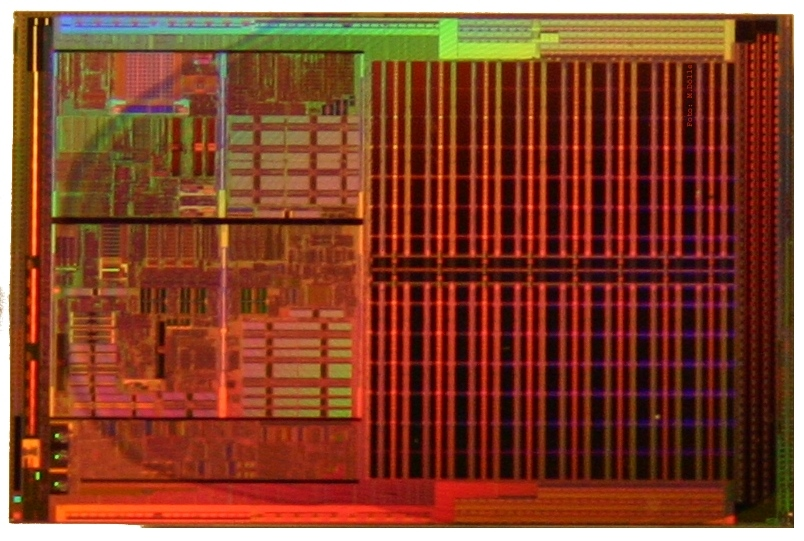
\includegraphics[width=3cm]{../intro/Opteron-die.jpg}};
\node[below=-2pt of cpu] {processor};
\node[anchor=center,right=8cm of cpu] (memory) {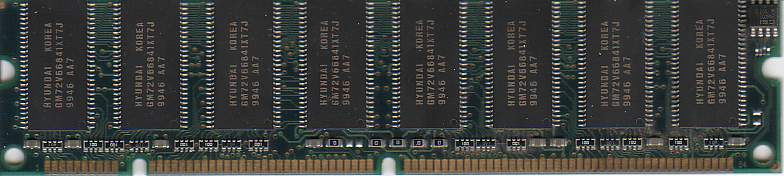
\includegraphics[height=0.75cm,angle=90]{../intro/SDRAM.jpg}};
\node[below=0pt of memory] {memory};

\onslide<1-3|handout:0>{
    \draw[latex-latex, line width=3pt] (cpu) -- (memory);
}
\coordinate (middleBus) at ($(cpu)!.5!(memory)$);


\onslide<3|handout:0>{
    \node[my callout2=middleBus,align=left] at ($(middleBus) + (-3cm,2cm)$) {bus \\ send address + send or get data};
}

\onslide<4->{
    \node[smallBox,anchor=center,fill=white, align=center] (ioBridge) at (middleBus) {I/O \\ Bridge};
    \draw[latex-latex, line width=3pt] (cpu) -- (ioBridge);
    \draw[latex-latex, line width=3pt] (ioBridge) -- (memory);
    \coordinate (toIO) at ($(middleBus) + (0,-3cm)$);
    \draw[latex-latex, line width=3pt] (ioBridge) -- (toIO);
    \node[below=0pt of toIO, align=left] {to I/O devices \\ \small keyboard, mouse, wifi, \ldots};
    \coordinate (middleSysBus) at ($(cpu)!.5!(middleBus)$);
    \coordinate (middleMemBus) at ($(memory)!.5!(middleBus)$);
    \coordinate (middleIOBus) at ($(middleBus)!.5!(toIO)$);
}
\onslide<5>{
    \node[my callout2=middleSysBus,align=left] at ($(middleSysBus) + (0,2cm)$) {bus \\ send address + send or get data \\ (machine code/text/number\ldots)};
}
\onslide<6-9>{
    \node[my callout2=middleSysBus,align=left] at ($(middleSysBus) + (0,2cm)$) {CPU: send PC: {\tt 0x04000}};
    \node[my callout2=middleMemBus,align=left] at ($(middleMemBus) + (-3cm,1cm)$) {MEM: send machine code: {\tt pushq \%rbp}};
}
\onslide<8-9>{
    \node[my callout2=middleSysBus,align=left] at ($(middleMemBus) + (0,-1cm)$) {MEM: stored it};
}
\onslide<9>{
    \node[my callout2=middleSysBus,align=left] at ($(middleSysBus) + (-1,-2cm)$) {CPU: next PC: {\tt 0x04001}};
}
\onslide<7-9>{
    \node[my callout2=middleSysBus,align=left] at ($(middleSysBus) + (0,0cm)$) {CPU: send {\tt 0x7fff830} (stack), {\tt 0x1234} (rbp)};
}
\onslide<10>{
    \node[my callout2=middleSysBus,align=left] at ($(middleSysBus) + (-2,2cm)$) {CPU: send I/O request address: {\tt 0xf122003}};
    \node[my callout2=middleIOBus,align=left] at ($(middleIOBus) + (1cm,0)$) {I/O: send keystoke: ``a''};
}
\end{tikzpicture}
\imagecredit{Images: \\
             Single core Opteron 8xx die: Dg2fer at the German language Wikipedia, via Wikimedia Commons \\
             SDRAM by Arnaud 25, via Wikimedia Commons}
\end{frame}



\subsection{Goals (if you don't care about HW)}

\begin{frame}<1>[label=goals]{goals/other topics}
    \begin{itemize}
    \item understand how hardware works for\ldots{}
    \item \myemph<2>{program performance}
    \item \myemph<3>{what compilers are/do}
    \item \myemph<4>{weird program behaviors} (segfaults, etc.)
    \end{itemize}
\end{frame}

\againframe<2>{goals}

\begin{frame}{program performance}
    \begin{itemize}
    \item naive model:
        \begin{itemize}
        \item one instruction = one time unit
        \end{itemize}
    \item number of instructions matters, but \ldots
    \end{itemize}
\end{frame}

\begin{frame}{program performance: issues}
    \begin{itemize}
    \item \myemph{parallelism}
        \begin{itemize}
        \item fast hardware is parallel
        \item needs multiple things to do
        \end{itemize}
    \item \myemph{caching}
        \begin{itemize}
        \item accessing things recently accessed is faster
        \item need reuse of data/code
        \end{itemize}
    \item (more in other classes: \myemph{algorithmic} efficiency)
    \end{itemize}
\end{frame}

\againframe<3>{goals}

\begin{frame}{what compilers are/do}
    \begin{itemize}
    \item understanding weird compiler/linker rrors
    \item if you want to make compilers
    \item debugging applications
    \end{itemize}
\end{frame}

\againframe<4>{goals}

\begin{frame}{weird program behaviors}
    \begin{itemize}
    \item what is a segmentation fault really?
    \item how does the operating system interact with programs?
    \item if you want to handle them --- writing OSs
    \end{itemize}
\end{frame}


\section{Logistics}
\begin{frame}{lectures and labs attendance} 
    \begin{itemize}
    \item we won't check lecture/lab attendance
    \vspace{.5cm}
    \item lectures will be recorded (assuming not tech. difficulties)
    \item remote submission of labs is possible
    \end{itemize}
\end{frame}

\begin{frame}{not attending lectures?}
    \begin{itemize}
    \item if you rely on the lecture recordings, I recommend\ldots
    \vspace{.5cm}
    \item \textit{a regular schedule of watching them}
    \item \textit{pausing+trying to answer in-lecture questions}
    \item \textit{writing down} questions you have
    \begin{itemize}
        \item \ldots and asking them in Piazza and/or office hours and/or lab
    \end{itemize}
    \end{itemize}
\end{frame}

\begin{frame}{coursework}
\begin{itemize}
    \item labs --- grading: full credit if threshold amount completed
        \begin{itemize}
        \item threshold often somewhat less than full lab
        \item collaboration permitted
        \end{itemize}
    \item homework assignments --- introduced by lab (mostly)
        \begin{itemize}
        \item due at 9:30am lab day
        \item \myemph<2>{complete individually}
        \end{itemize}
    \item weekly quizzes
    \item final exam
\end{itemize}
\end{frame}

\begin{frame}{textbook}
    \begin{itemize}
    \item Computer Systems: A Programmer's Perspective
    \item recommended --- HCL assignments follow pretty closely
    \item (useful, but less important for other topics)
    \end{itemize}
\begin{tikzpicture}[overlay,remember picture]
    \node[anchor=north east] at ([xshift=-.5cm,yshift=-1cm]current page.north east) {
        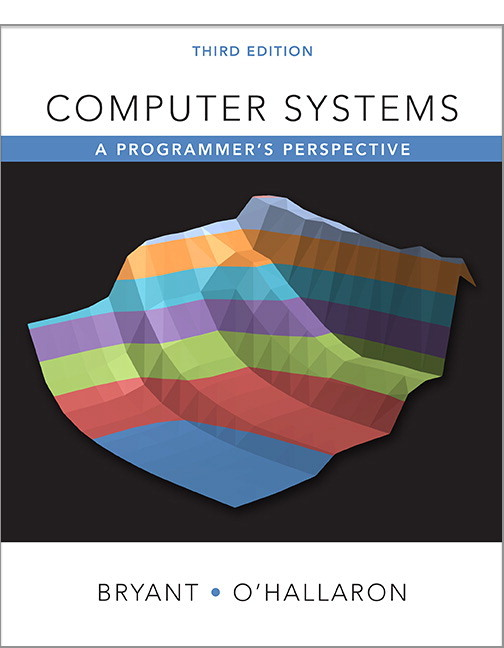
\includegraphics[width=3cm]{../intro/csapp3e-cover}
    };
\end{tikzpicture}
\end{frame}

\begin{frame}{on lecture/lab/HW synchronization}
    \begin{itemize}
        \item labs/HWs not quite synchronized with lectures
        \item main problem: want to cover material \textbf{before you need it} in lab/HW
    \end{itemize}
\end{frame}

% FIXME: textbook picture

\begin{frame}{quizzes?}
    \begin{itemize}
    \item linked off course website (demo Thursday)
    \item released Thursday night, due Tuesday before \textit{first} lecture
    \item from lecture that week
    \vspace{.5cm}
    \item two lowest quiz grades dropped
    \end{itemize}
\end{frame}

\begin{frame}{late policy}
    \begin{itemize}
    \item exceptional circumstance? contact us.
    \item otherwise, for \myemph{homeworks only}:
        \begin{itemize}
        \item -10\% 0 to 48 hours late
        \item -15\% 48 to 72 hours late
        \item -100\% otherwise
        \end{itemize}
    \item late quizzes, labs: no
        \begin{itemize}
        \item we release answers
        \item talk to me if illness, etc.
        \end{itemize}
    \end{itemize}
\end{frame}

\begin{frame}{getting help tools}
    \begin{itemize}
    \item non-real-time help: Piazza (discussion forum)
    \item labs: in person, specified location
    \item office hours: specified on website, calendar
        \begin{itemize}
        \item some in-person, some remote
        \item online queue for TA help (might not be used in smaller rooms)
        \end{itemize}
    \end{itemize}
\end{frame}

\begin{frame}{office hour format}
    \begin{itemize}
    \item current plan: mix of remote (Discord) + in-person
    \item generally: believe in-person usually more efficient
        \begin{itemize}
        \item but some other practicalities
        \end{itemize}
    \item which it is will be noted on schedule
        \begin{itemize}
        \item never in-person+remote at smae time
        \end{itemize}
    \item common office hour queue
    \end{itemize}
\end{frame}

\begin{frame}{on the office hour queue}
    \begin{itemize}
    \item except for first three slots, queue is sorted by last time helped
    \item we may reset those first three slots between office hours
    \vspace{.5cm}
    \item goal 1: being on the queue overnight won't help you
    \item goal 2: try to spread out the TA help
    \end{itemize}
\end{frame}

\begin{frame}{your TODO list}
    \begin{itemize}
    \item department account and/or C environment working
        \begin{itemize}
        \item department accounts should happen by this weekend
        \end{itemize}
    \item before lab next week
    \end{itemize}
\end{frame}

\begin{frame}{upcoming lab/HW}
    \begin{itemize}
    \item bomblab/hw:
    \item using debugger/disassembler, \\ figure out ``correct'' input for a program
    \item may want to review x86-64 assembly from CS 2150
        \begin{itemize}
        \item (or see textbook chapter/writeup linked off assignment)
        \end{itemize}
    \end{itemize}
\end{frame}

\section{Backup slides}

\begin{frame}{grading}
    \begin{itemize}
    \item Quizzes: 30\%
    \item Homeworks: 40\%
    \item Labs: 15\%
    \item Final Exam: 15\%
    \end{itemize}
\end{frame}

\begin{frame}
\end{frame}


\begin{frame}{quiz demo}
\end{frame}

\section{Memory and Endianness}

\usetikzlibrary{fit,matrix,positioning,shapes.callouts}

\newcommand{\memoryPicture}{
\matrix (memoryWithLabels) [matrix of nodes,
    row sep=2mm,
    inner sep=0mm,
    font=\small\ttfamily,
    nodes={text depth=0pt,inner sep=0.2mm,inner xsep=1mm},
    column 1/.style={align=right,column sep=2mm},
    column 2/.style={align=left,minimum width=1cm},
    row 1/.style={font=\small\bfseries}] {
        address \& value \\
        0xFFFFFFFF  \& 0x14\\
        0xFFFFFFFE  \& 0x45\\
        0xFFFFFFFD  \& 0xDE\\
        \ldots  \& \ldots \\
        0x00042006  \& 0x06\\
        0x00042005  \& 0x05\\
        0x00042004  \& 0x04\\
        0x00042003  \& 0x03\\
        0x00042002  \& 0x02\\
        0x00042001  \& 0x01\\
        0x00042000  \& 0x00\\
        0x00041FFF  \& 0x03\\
        0x00041FFE  \& 0x60\\
        \ldots  \& \ldots \\
        0x00000002  \& 0xFE\\
        0x00000001  \& 0xE0\\
        0x00000000  \& 0xA0\\
};
\draw[black!80!white,line width=1pt] (memoryWithLabels-2-2.north west) rectangle (memoryWithLabels-4-2.south east);
\draw[black!80!white,line width=1pt] (memoryWithLabels-6-2.north west) rectangle (memoryWithLabels-14-2.south east);
\draw[black!80!white,line width=1pt] (memoryWithLabels-16-2.north west) rectangle (memoryWithLabels-18-2.south east);
\foreach \x in {3,4,7,8,...,14,17,18} {
    \draw[black!80!white,line width=1pt] (memoryWithLabels-\x-2.north west) -- (memoryWithLabels-\x-2.north east);
}
}

\newcommand{\memoryPictureInverted}[1]{
\matrix (memoryWithLabelsInverted) [matrix of nodes,
    row sep=2mm,
    inner sep=0mm,
    font=\small\ttfamily,
    nodes={text depth=0pt,inner sep=0.2mm,inner xsep=1mm},
    column 1/.style={align=right,column sep=2mm},
    column 2/.style={align=left,minimum width=1cm},
    row 1/.style={font=\small\bfseries},anchor=north west] at #1 {
        address \& value \\
        0x00000000  \& 0xA0\\
        0x00000001  \& 0xE0\\
        0x00000002  \& 0xFE\\
        \ldots  \& \ldots \\
        0x00041FFE  \& 0x60\\
        0x00041FFF  \& 0x03\\
        0x00042000  \& 0x00\\
        0x00042001  \& 0x01\\
        0x00042002  \& 0x02\\
        0x00042003  \& 0x03\\
        0x00042004  \& 0x04\\
        0x00042005  \& 0x05\\
        0x00042006  \& 0x06\\
        \ldots  \& \ldots \\
        0xFFFFFFFD  \& 0xDE\\
        0xFFFFFFFE  \& 0x45\\
        0xFFFFFFFF  \& 0x14\\
};
\draw[black!80!white,line width=1pt] (memoryWithLabelsInverted-2-2.north west) rectangle (memoryWithLabelsInverted-4-2.south east);
\draw[black!80!white,line width=1pt] (memoryWithLabelsInverted-6-2.north west) rectangle (memoryWithLabelsInverted-14-2.south east);
\draw[black!80!white,line width=1pt] (memoryWithLabelsInverted-16-2.north west) rectangle (memoryWithLabelsInverted-18-2.south east);
\foreach \x in {3,4,7,8,...,14,17,18} {
    \draw[black!80!white,line width=1pt] (memoryWithLabelsInverted-\x-2.north west) -- (memoryWithLabelsInverted-\x-2.north east);
}
}

%FIXME: Memory picture
\begin{frame}{memory}
\begin{tikzpicture}
\memoryPicture
\onslide<2>{
    \node[align=left,my callout2=memoryWithLabels-2-2.east] {\myemph{array of bytes} (byte = 8 bits) \\
                                                 CPU interprets based on how accessed};
}
\onslide<3>{
    \memoryPictureInverted{([xshift=3cm]memoryWithLabels.north east)}
}
\end{tikzpicture}
\end{frame}


% FIXME: Endianness picture
\begin{frame}[fragile,label=endiannes]{endianness}
\begin{tikzpicture}
\memoryPicture
\node[right=10mm of memoryWithLabels-2-2] (code) {
\begin{minipage}{4cm}
\begin{minted}{c}
int *x = (int*)0x42000;
printf("%d\n", *x);
\end{minted}
\end{minipage}
};
%\node[right=1mm of memoryWithLabels-12-2] {\Huge$\Leftarrow$};
\onslide<2->{
    \node[fit=(memoryWithLabels-9-2) (memoryWithLabels-12-2),rectangle,draw=orange!70!black,line width=1mm] {};
}
\onslide<3->{
    \node[below=.2cm of code,xshift=10mm] (le) {\ttfamily 0x030201\myemph{00} $=$};
    \node[right=0cm of le] (leDec) {50462976};
    \node[below=2cm of le] (be) {\ttfamily 0x\myemph{00}010203 $=$};
    \node[right=0cm of be] (beDec) {66051};
}
\begin{pgfonlayer}{bg}
\onslide<4->{
    \node[below=.1cm of le,xshift=.5cm,fill=blue!20, align=center] {little endian \\ (least significant byte has lowest address)};
    \node[fit=(leDec),inner sep=1mm,draw=blue!70!black,fill=blue!10, line width=1mm] (boxLe) {};
    \node[below=.1cm of be,xshift=.5cm,fill=green!20, align=center] {big endian \\ (most significant byte has lowest address)};
    \node[fit=(beDec),inner sep=1mm,draw=green!70!black,fill=green!10, line width=1mm] (boxBe) {};
}
\end{pgfonlayer}
\onslide<5->{
}
\end{tikzpicture}
\end{frame}



\subsection{exercise}
\usetikzlibrary{decorations.pathreplacing,matrix}
\begin{frame}<1-5>[fragile,label=endianEx]{exercise}
\lstset{
    language=C++,style=smaller,
    moredelim=**[is][\btHL<2>]{@2}{2@},
    moredelim=**[is][\btHL<3>]{@3}{3@},
    moredelim=**[is][\btHL<4>]{@4}{4@},
}
\begin{lstlisting}
unsigned char buffer[8] =
    { 0, 0, /* ..., */ 0 };
/* uint32_t = 32-bit unsigned int */
uint32_t value1 = 0x12345678;
uint32_t value2 = 0x9ABCDEF0;
@2unsigned char *ptr_value1 = (unsigned char *) &value1;2@
@2unsigned char *ptr_value2 = (unsigned char *) &value2;2@
@3for (int i = 0; i < 4; ++i) {3@ /* copy value1/2 into buffer */
    @3buffer[i] = ptr_value1[i];3@
    @3buffer[i+4] = ptr_value2[i];3@
@3}3@
@4for (int i = 0; i < 4; ++i) {4@ /* copy buffer[1..5] into value1 */
    @4ptr_value1[i] = buffer[i+1];4@
@4}4@
\end{lstlisting}
What is \texttt{value1} after this runs on a little-endian system? \\
\begin{tabular}{lll}
\textbf{A.} \texttt{0x0F654321} & \textbf{B.} \texttt{0x123456F0}  & \textbf{C.}  \texttt{0x3456789A} \\
\textbf{D.} \texttt{0x345678F0} & \textbf{E.} \texttt{0x9A123456} & \textbf{F.} \texttt{0x9A785634} \\
\textbf{G.} \texttt{0xF0123456} & \textbf{H.} \texttt{0xF2345678} & \textbf{I.} something else \\
\end{tabular}
\begin{tikzpicture}[overlay,remember picture]
\coordinate (base) at ([xshift=-1cm,yshift=-1.5cm]current page.north east);
\matrix[tight matrix,nodes={text width=.45cm},anchor=north east,label={[label distance=.5cm]north:buffer}] (buffer) at (base) {
    ~ \& ~ \& ~ \& ~ \&
    ~ \& ~ \& ~ \& ~ \\
};
\begin{visibleenv}<3->
    \draw[decorate,decoration={brace},very thick,alt=<2>{red}]
        ([yshift=1mm,xshift=1mm]buffer-1-1.north west) --
        ([yshift=1mm,xshift=-1mm]buffer-1-4.north east)
        node[midway,above,font=\tt\fontsize{9}{10}\selectfont] {0x12345678};

    \draw[decorate,decoration={brace},very thick,alt=<2>{red}]
        ([yshift=1mm,xshift=1mm]buffer-1-5.north west) --
        ([yshift=1mm,xshift=-1mm]buffer-1-8.north east)
        node[midway,above,font=\tt\fontsize{9}{10}\selectfont] {0x9ABCDEF0};
\end{visibleenv}
\begin{pgfonlayer}{bg}
    \begin{visibleenv}<4->
        \draw[blue,very thick,fill=blue!10] (buffer-1-2.north west) rectangle (buffer-1-5.south east);
        \draw[blue,->,very thick] (buffer-1-4.south west) -- ++ (0cm, -.5cm) node[below,font=\tt\fontsize{9}{10}\selectfont] {value1};
    \end{visibleenv}
\end{pgfonlayer}
\end{tikzpicture}
\end{frame}
 % FIXME: soln slide

\subsubsection{explanation}
\usetikzlibrary{decorations.pathreplacing,matrix}
\begin{frame}[fragile,label=endianExViz]{exercise visualization}
\lstset{
    language=C++,style=smaller,
    moredelim=**[is][{\btHL<2>[fill=green!30]}]{@a}{a@},
    moredelim=**[is][{\btHL<2>[fill=blue!30]}]{@b}{b@},
    moredelim=**[is][\btHL<3>]{@3}{3@},
    moredelim=**[is][\btHL<4>]{@4}{4@},
}
\vspace{1.1cm}
\tikzmark{copy1}
\begin{lstlisting}
for (int i = 0; i < 4; ++i) { /* copy value1/2 into buffer */
    @abuffer[i] = ptr_value1[i];a@ @bbuffer[i+4] = ptr_value2[i];b@
}
\end{lstlisting}
\vspace{1cm}
\tikzmark{copy2}
\begin{lstlisting}
for (int i = 0; i < 4; ++i) { /* copy buffer[1..5] into value1 */
    @3ptr_value1[i] = buffer[i+1];3@
}
\end{lstlisting}
\tikzmark{copy3}
\begin{tikzpicture}[overlay,remember picture]
\tikzset{
    small box/.style={draw,thick,font=\small},
    small label/.style={font=\small},
    my array/.style={
        tight matrix,
        nodes={text width=.7cm,text depth=0mm,font=\tt\small,align=center},
        row 2/.style={
            nodes={font=\fontsize{9}{10}\selectfont,draw=none,align=center},
        }
    },
    real value/.style={font=\small\tt\selectfont},
}
\matrix[my array,anchor=north west,label={[small label]north:value1 {\scriptsize (bytes in hex)}}] (value1 init) at ([yshift=1.2cm]pic cs:copy1) {
    78 \& 56 \& 34 \& 12 \\
    0 \& 1 \& 2 \& 3 \\
};
\draw[very thick,decorate,decoration={brace,mirror}] (value1 init-2-1.south west) -- (value1 init-2-4.south east)
    node[midway,below,real value] {0x12345678};
\matrix[my array,anchor=north west,label={[small label]north:value2 {\scriptsize (bytes in hex)}}] (value2 init) at ([xshift=.25cm]value1 init.north east) {
    F0 \& DE \& BC \& 9A \\
    0 \& 1 \& 2 \& 3 \\
};
\draw[very thick,decorate,decoration={brace,mirror}] (value2 init-2-1.south west) -- (value2 init-2-4.south east)
    node[midway,below,real value] {0x9ABCDEF0};
\matrix[my array,anchor=north west,label={[small label]north:buffer}] (buffer init) at ([xshift=.25cm]value2 init.north east) {
    ? \& ? \& ? \& ? \& ? \& ? \& ? \& ? \\
    0 \& 1 \& 2 \& 3 \& 4 \& 5 \& 6 \& 7 \\
};

\matrix[my array,anchor=north west,label={[small label]north:value1}] (value1 copy1) at ([yshift=1.2cm]pic cs:copy2) {
    78 \& 56 \& 34 \& 12 \\
    0 \& 1 \& 2 \& 3 \\
};
\draw[very thick,decorate,decoration={brace,mirror}] (value1 copy1-2-1.south west) -- (value1 copy1-2-4.south east)
    node[midway,below,real value] {0x12345678};
\matrix[my array,anchor=north west,label={[small label]north:value2}] (value2 copy1) at ([xshift=.25cm]value1 copy1.north east) {
    F0 \& DE \& BC \& 9A \\
    0 \& 1 \& 2 \& 3 \\
};
\draw[very thick,decorate,decoration={brace,mirror}] (value2 copy1-2-1.south west) -- (value2 copy1-2-4.south east)
    node[midway,below,real value] {0x9ABCDEF0};
\matrix[my array,anchor=north west,label={[small label]north:buffer}] (buffer copy1) at ([xshift=.25cm]value2 copy1.north east) {
    78 \& 56 \& 34 \& 12 \& F0 \& DE \& BC \& 9A \\
    0 \& 1 \& 2 \& 3 \& 4 \& 5 \& 6 \& 7 \\
};

\matrix[my array,anchor=north west,label={[small label]north:value1}] (value1 copy2) at ([yshift=0cm]pic cs:copy3) {
    56 \& 34 \& 12 \& F0 \\
    0 \& 1 \& 2 \& 3 \\
};
\draw[very thick,decorate,decoration={brace,mirror}] (value1 copy2-2-1.south west) -- (value1 copy2-2-4.south east)
    node[midway,below,real value] {0xF01234\myemph<4>{56}};
\matrix[my array,anchor=north west,label={[small label]north:value2}] (value2 copy2) at ([xshift=.25cm]value1 copy2.north east) {
    F0 \& DE \& BC \& 9A \\
    0 \& 1 \& 2 \& 3 \\
};
\draw[very thick,decorate,decoration={brace,mirror}] (value2 copy2-2-1.south west) -- (value2 copy2-2-4.south east)
    node[midway,below,real value] {0x9ABCDEF0};
\matrix[my array,anchor=north west,label={[small label]north:buffer}] (buffer copy2) at ([xshift=.25cm]value2 copy2.north east) {
    78 \& 56 \& 34 \& 12 \& F0 \& DE \& BC \& 9A \\
    0 \& 1 \& 2 \& 3 \& 4 \& 5 \& 6 \& 7 \\
};
\begin{visibleenv}<2>
    \path[draw=green!50!black,very thick,fill=green,fill opacity=0.1]
        (value1 copy1-1-1.north west) rectangle (value1 copy1-1-4.south east);
    \path[draw=green!50!black,very thick,fill=green,fill opacity=0.1]
        (buffer copy1-1-1.north west) rectangle (buffer copy1-1-4.south east);

    \path[draw=blue!50!black,very thick,fill=blue,fill opacity=0.1]
        (value2 copy1-1-1.north west) rectangle (value2 copy1-1-4.south east);
    \path[draw=blue!50!black,very thick,fill=blue,fill opacity=0.1]
        (buffer copy1-1-5.north west) rectangle (buffer copy1-1-8.south east);
\end{visibleenv}
\begin{visibleenv}<3>
    \path[draw=red!50!black,very thick,fill=red,fill opacity=0.1]
        (value1 copy2-1-1.north west) rectangle (value1 copy2-1-4.south east);
    \path[draw=red!50!black,very thick,fill=red,fill opacity=0.1]
        (buffer copy2-1-2.north west) rectangle (buffer copy2-1-5.south east);
\end{visibleenv}
\begin{visibleenv}<4>
    \path[draw=red!50!black,very thick,fill=red,fill opacity=0.1]
        (value1 copy2-1-1.north west) rectangle (value1 copy2-1-1.south east);
\end{visibleenv}
\begin{pgfonlayer}{bg}
\end{pgfonlayer}
\end{tikzpicture}
\end{frame}
 % FIXME: soln slide

